\documentclass[class=article, crop=false]{standalone}
\usepackage[subpreambles=true]{standalone}
\usepackage{import}
\usepackage[T1]{fontenc}
\usepackage[utf8]{inputenc}
\usepackage[english, danish]{babel}
\usepackage{graphicx,wrapfig,lipsum}

\begin{document}
    Jar-filen kan også åbnes direkte fra GitHub: \\
    1. Klik følgende link: \url{https://github.com/ArmandasRokas/matador/releases}\\
2. Download 44\_final.jar, som er understreget på nedenstående billede:
    \begin{figure}[H]
        \centering
        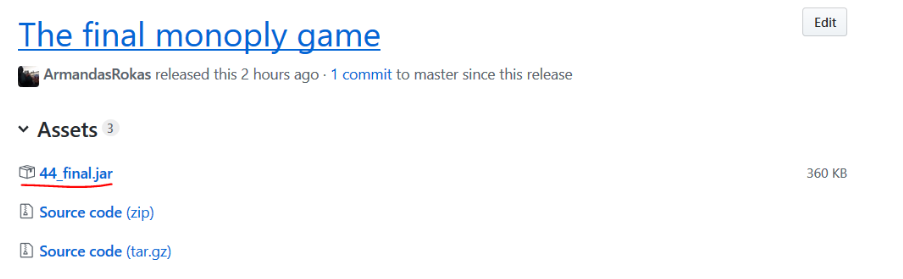
\includegraphics[scale=0.7]{pics/vejledning}
        \caption{Github release}\label{fig:vejledning}
    \end{figure}
3. Kør filen.

\end{document}